%/**************************************
% * Displaying Wind Vectors in ArcMap  *
%/**************************************
\documentclass[12pt]{article}
%\documentstyle{report}
\usepackage{float}
\usepackage{graphicx}
\usepackage[margin=1in]{geometry}
%\usepackage{subfig}


\graphicspath{{images/}}

\usepackage[utf8]{inputenc}
\usepackage[english]{babel}
\usepackage[parfill]{parskip}
\usepackage{datetime}
\usepackage{hyperref}
\hypersetup{
	colorlinks=true,
	urlcolor=blue,
  }
\urlstyle{same}
%\newdate{date}{26}{04}{2018}
%\date{\displaydate{date}}
%\usepackage{subcaption} 
\usepackage{subfig}
\usepackage{dirtytalk}
\usepackage{multirow}
\usepackage{booktabs}
\usepackage{enumitem}
\usepackage{nameref}

\usepackage{fancyhdr}
\pagestyle{fancy}
\fancyhf{}
\rhead{Displaying and Rotating WindNinja-Derived
Wind Vectors in ArcMap 10.5}
\cfoot{\thepage}

\newcommand\vn{3.6.0}

\begin{document}
\begin{titlepage}
    \centering
    {\Huge
        Displaying and Rotating WindNinja-Derived
Wind Vectors in ArcMap 10.5
    }
    \vfill
    {\Large
    Chuck McHugh\\ RMRS, Fire Sciences Lab, Missoula, MT, 406-829-6953, \href{mailto:cmchugh@fs.fed.us}{cmchugh@fs.fed.us}
    }
    \vfill
    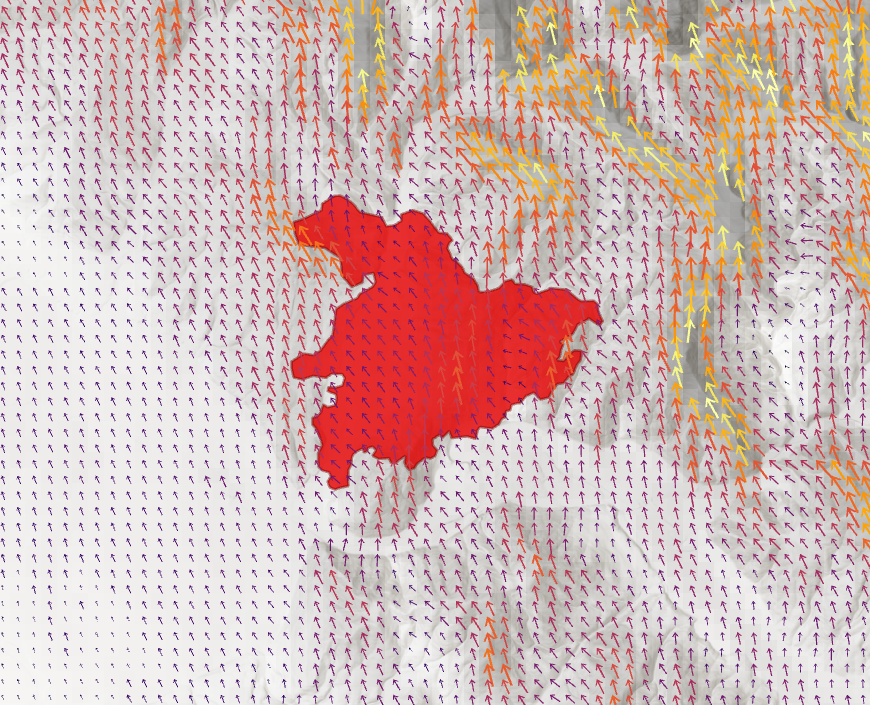
\includegraphics[scale=0.6]							{arc_00.png}
    \vfill
  	{\Huge
	  3/25/2020 %Date Last Edited
  	}
    \vfill
\end{titlepage}

\section*{Displaying WindNinja-generated gridded wind vectors}
Data requirements are an ArcMap shapefile format. The shapefile generated during the WindNinja process will
contain five data fields in the associated .DBF file (Figure \ref{fig:Figure1}).

\begin{figure}[H]
	\centering
	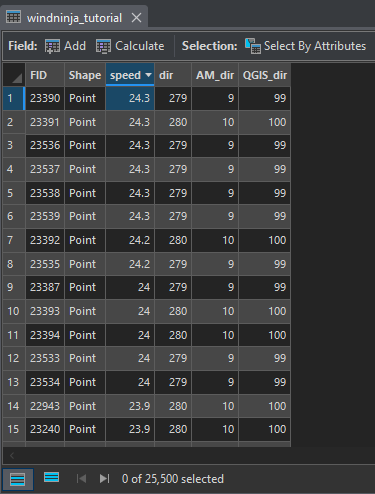
\includegraphics[scale=0.9]{arc_1.png}
	\caption{Attribute table for WindNinja-generated shapefile as displayed in ArcMap.}
	\label{fig:Figure1}
\end{figure}

\begin{enumerate}[label=(\alph*)]
\item \textbf{FID:} Feature ID, a unique number assigned to that point by ArcMap.
\item \textbf{Shape:} Point indicates that the feature type for the shapefile is a point
\item \textbf{speed:} WindNinja-generated wind speed at the specified output height and in the specified output units.
\item \textbf{dir:} WindNinja-generated azimuth direction the wind is coming from in degrees (e.g., 0 degrees is wind from
the north).
\item \textbf{AM\_dir:} WindNinja-manipulated value required for use in ArcMap for display purposes.
\item \textbf{QGIS\_dir:}WindNinja-manipulated value required for use in QGIS for display purposes
\end{enumerate}
\subsection*{Steps:}
\begin{enumerate}
\item Open ArcMap and load other data coverages and fire perimeter files of interest.
\item Load the ArcMap WindNinja shapefile for the fire of interest. The wind vector grid will appear on the
coverage as individual points (Figure~\ref{fig:Figure2}).

\begin{figure}[H]
	\centering
	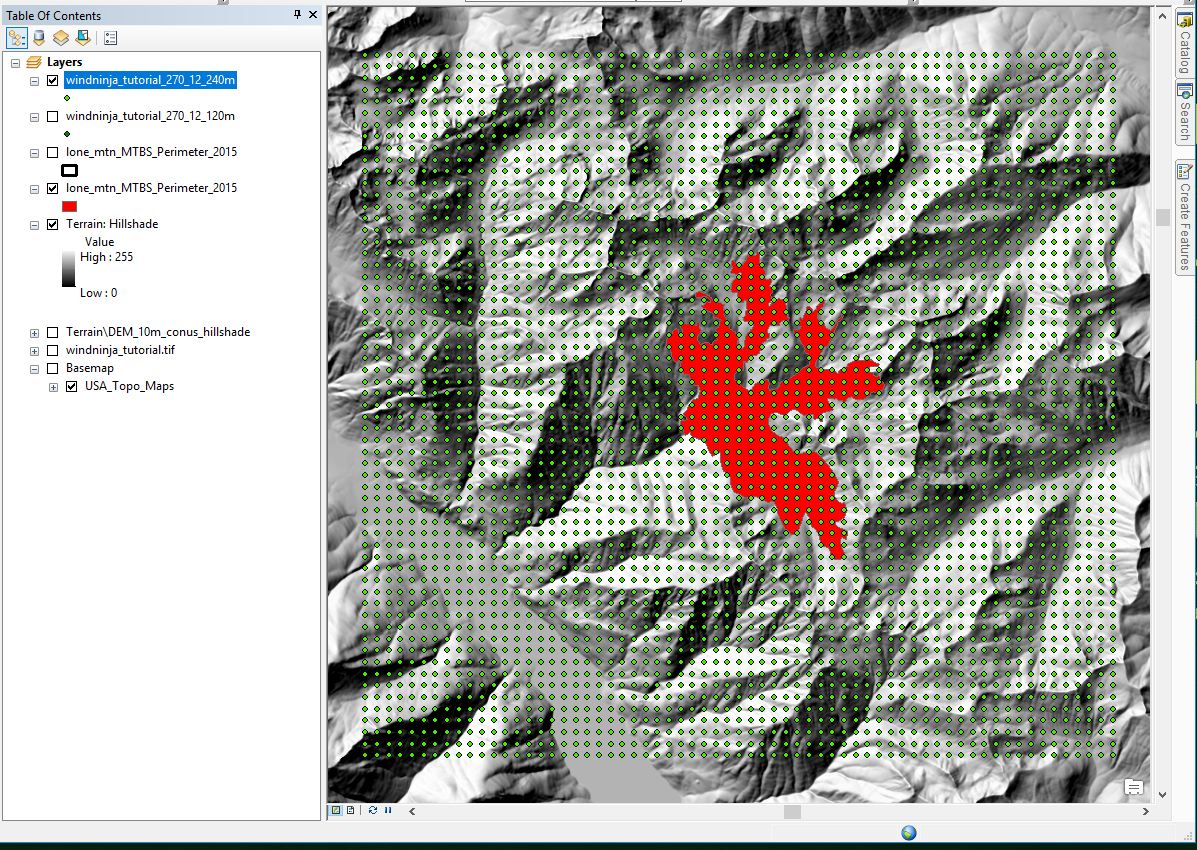
\includegraphics[scale=0.4]{arc_2.png}
	\caption{Example ArcMap project with WindNinja-generated shapefile as displayed in ArcMap prior to scaling and rotation of the
WindNinja-generated vectors.}
\label{fig:Figure2}

\end{figure}

\item After loading the file into the ArcMap project, double click on the layer name in the \textbf{Table of Contents} to
open the \textbf{Layer Properties.} This will open the dialog box in Figure 3.

\item Click on the \textbf{Symbology} tab (Figure~\ref{fig:Figure3}).

\begin{figure}[H]
	\centering
	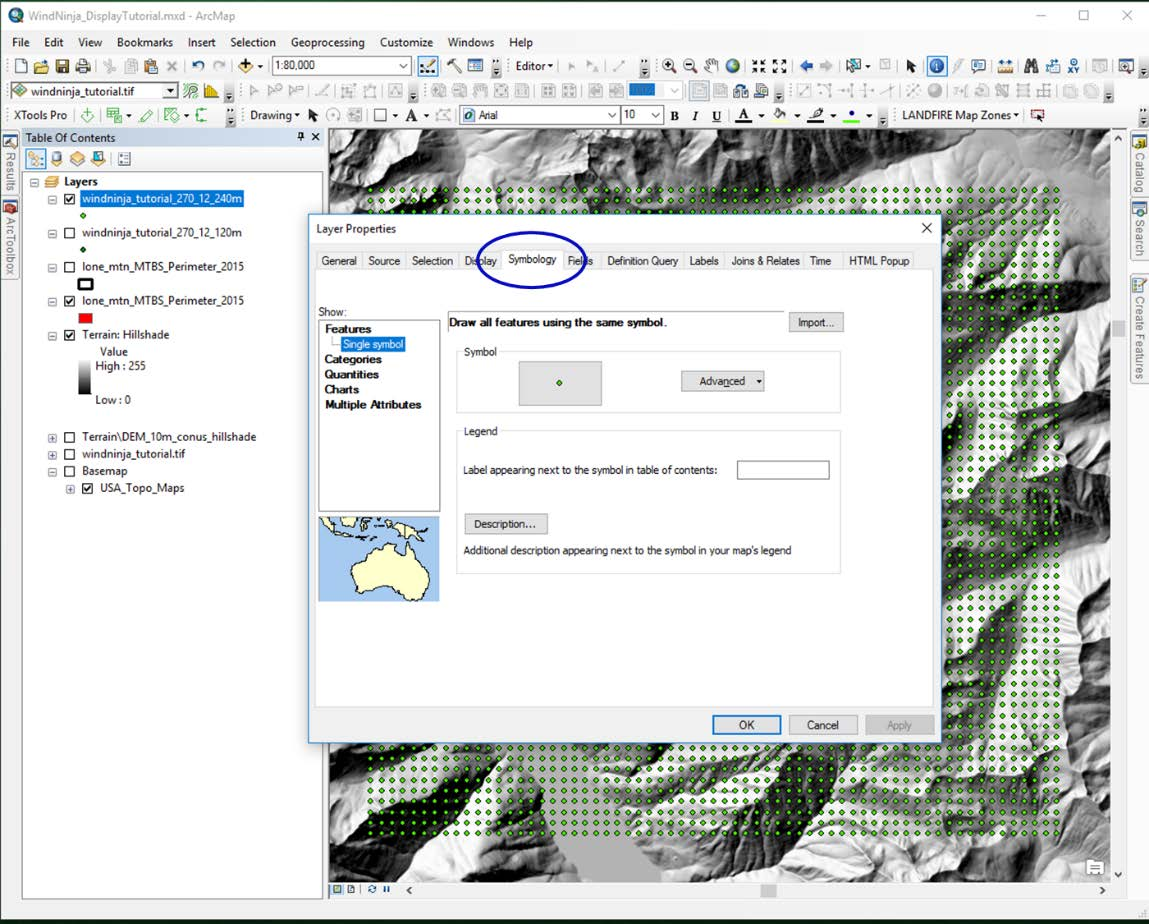
\includegraphics[scale=0.35]{arc_3.png}
	\caption{Layer Properties dialog box as displayed in ArcMap}
\label{fig:Figure3}
\end{figure}

\item In the \textbf{Show} pane on the left side of the dialog box, select \textbf{Quantities} then \textbf{Graduated symbols} (Figure~\ref{fig:Figure4}).

\begin{figure}[H]
	\centering
	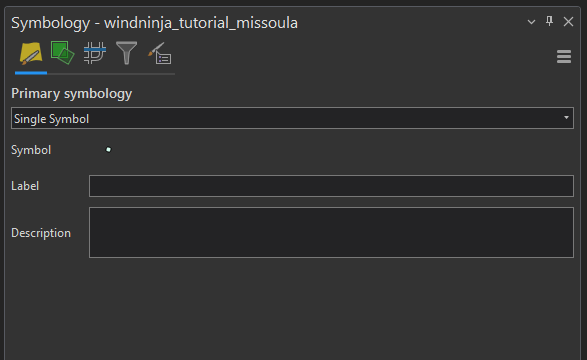
\includegraphics[scale=0.3]{arc_4.png}
	\caption{Changing the Symbol Size Range and choosing a new symbol set with arrows.}
\label{fig:Figure4}
\end{figure}

\item In the Value window click on the drop down arrow and select speed from the available options.

\begin{figure}[H]
	\centering
	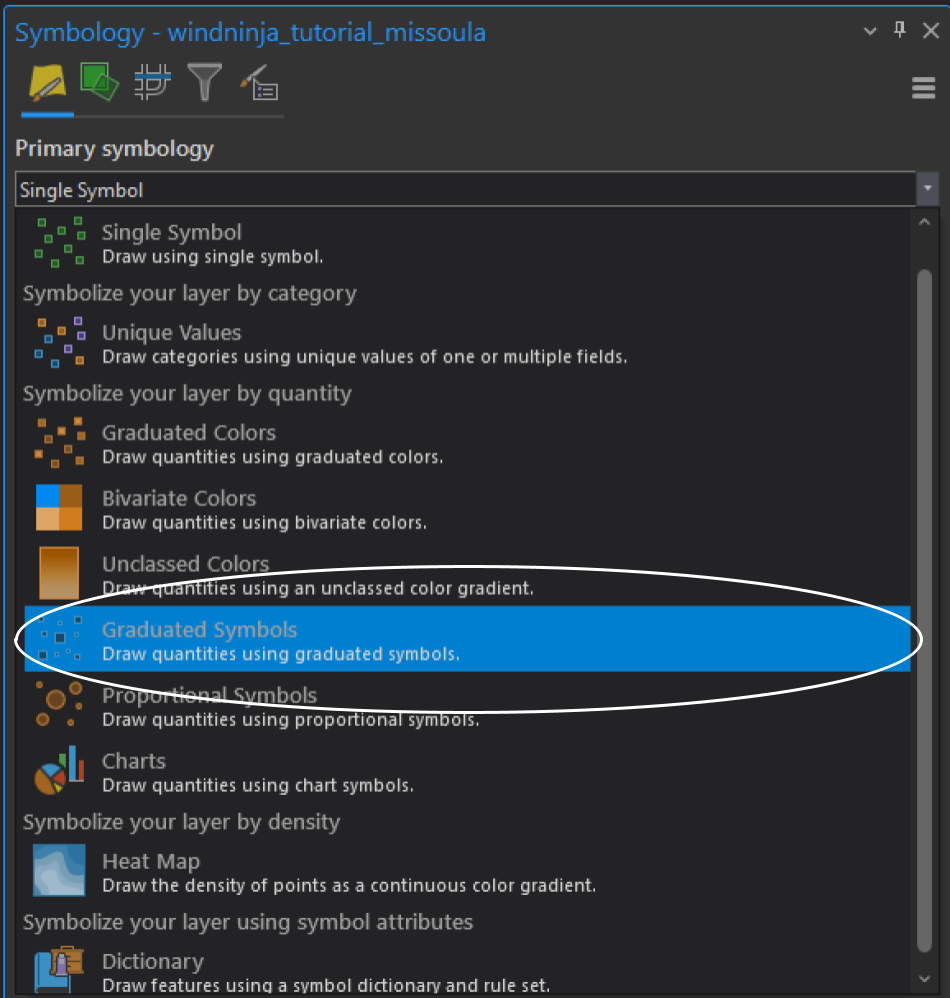
\includegraphics[scale=0.3]{arc_5.png}
	\caption{Selecting Quantities, Graduated Symbols, and Fields to speed.}
\label{fig:Figure5}
\end{figure}
\end{enumerate}
\textbf{Note: }The following Warning Message may appear depending on the number of records in the WindNinja shapefile.
Click on the OK button and the Warning Message will disappear. To change the number of records in ArcMap refer
to the~\nameref{section:appendix} of this document.

\begin{figure}[H]
	\centering
	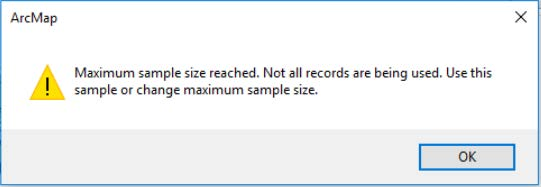
\includegraphics[scale=0.5]{arc_5_1.png}
%	\caption{Selecting Quantities, Graduated Symbols, and Fields to speed.}
\label{fig:Figure5_1}
\end{figure}

\begin{enumerate}[resume]
\item Select the display symbol and change the \textbf{Symbol Size} (Figure~\ref{fig:Figure6}). Enter a \textbf{Symbol Size} range (20 -30).
Arrows are not in the default symbol sets. To select an arrow to display you need to choose one of the
symbol sets that have arrows in it. This is done by clicking on the \textbf{Template} button (Figure ~\ref{fig:Figure6}).

\begin{figure}[H]
	\centering
	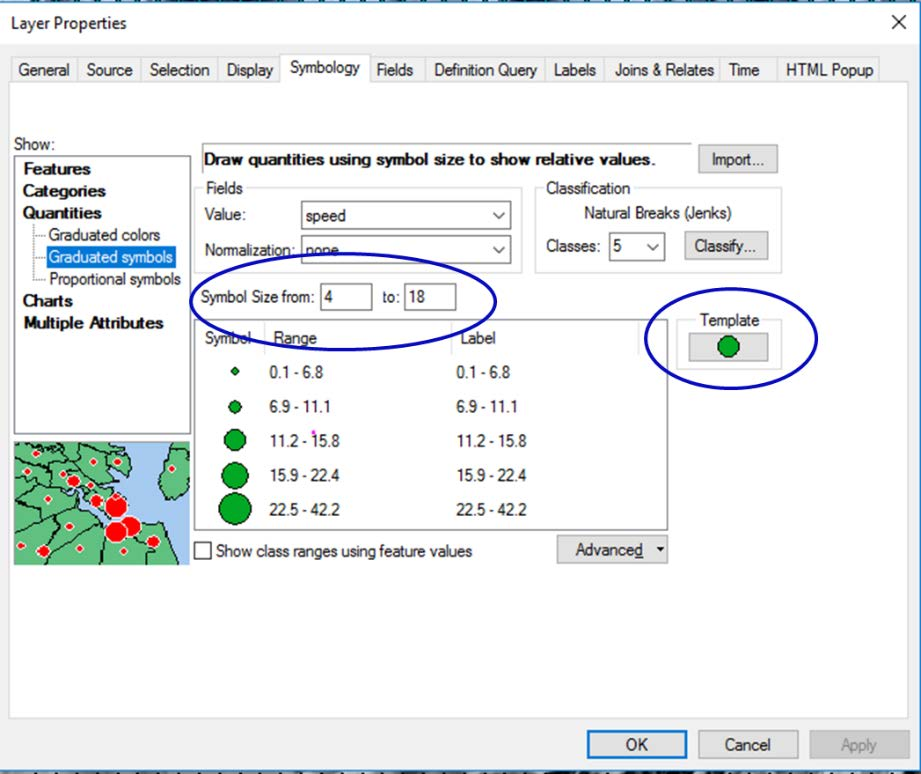
\includegraphics[scale=0.35]{arc_6.png}
	\caption{Select Template to access available symbol sets.}
\label{fig:Figure6}
\end{figure}

\item Select a symbol to represent the wind vectors (Figure~\ref{fig:Figure7}). In the \textbf{Symbol Selector Category}, type Wind then
enter. Scroll down until you see \textbf{Wind Speed Direction}.

\begin{figure}[H]
	\centering
	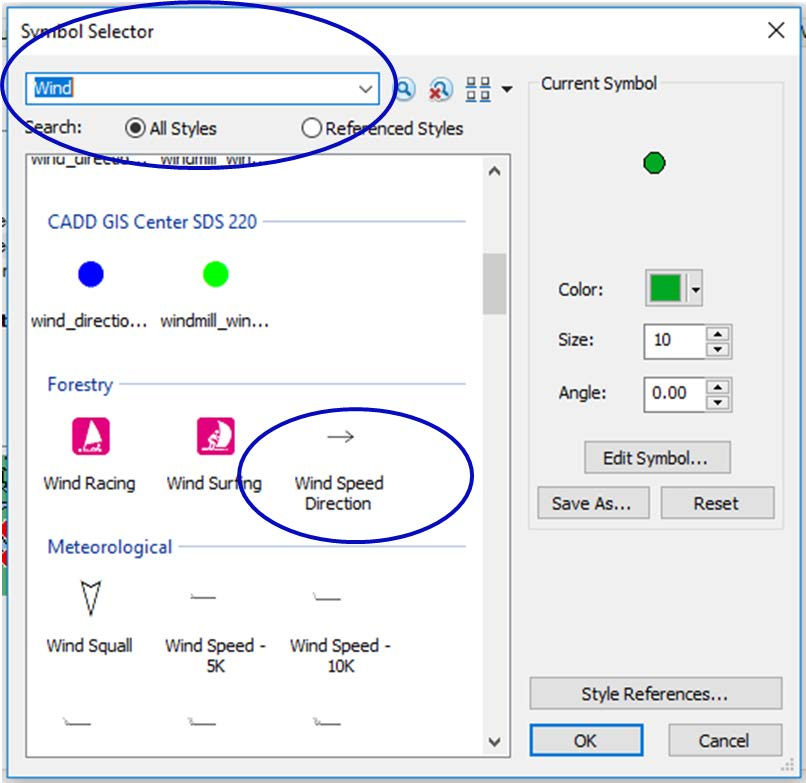
\includegraphics[scale=0.35]{arc_7.png}
	\caption{Symbol Selector dialog box.}
\label{fig:Figure7}
\end{figure}

\item Select the \textbf{Wind Speed Direction} symbol, click \textbf{OK} to return to the \textbf{Layer Properties}.

\item Click on the \textbf{Advanced $\rightarrow$ Rotation} button which will open the Rotation dialog box (Figure ~\ref{fig:Figure8}). Click on
the dropdown arrow and select \textbf{AM\_dir} to rotate the points from the available options and select
\textbf{Geographic} in the radio button for \textbf{Rotation Style} (Figure ~\ref{fig:Figure9}).

\begin{figure}[H]
	\centering
	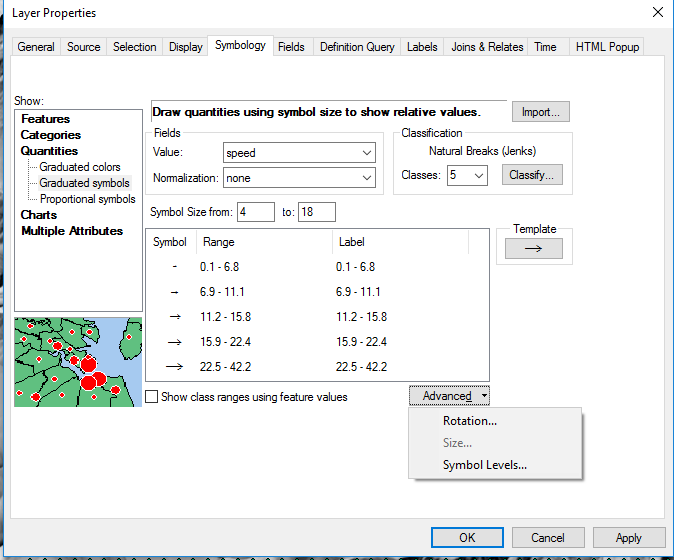
\includegraphics[scale=0.35]{arc_8.png}
	\caption{Select Advanced to access Rotation options.}
\label{fig:Figure8}
\end{figure}

\begin{figure}[H]
	\centering
	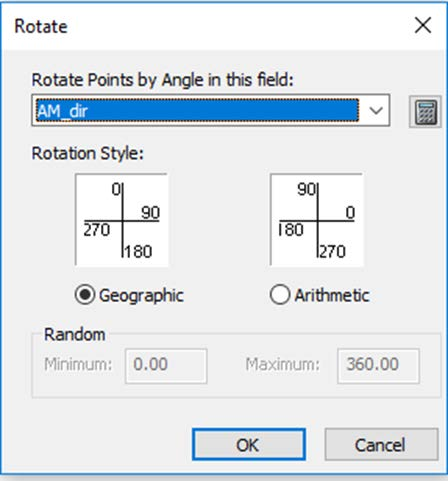
\includegraphics[scale=0.35]{arc_9.png}
	\caption{Rotation dialog box options.}
\label{fig:Figure9}
\end{figure}

\item Click \textbf{OK} to close the \textbf{Rotation} window and OK again to close the \textbf{Layer Properties} window.

\item The wind vectors will appear over the existing layers (Figure~\ref{fig:Figure10}).

\item Symbol colors can be changed by clicking on the individual symbols in the \textbf{Table of
Contents} for the respective shapefile (Figure~\ref{fig:Figure10}).

\begin{figure}[H]
	\centering
	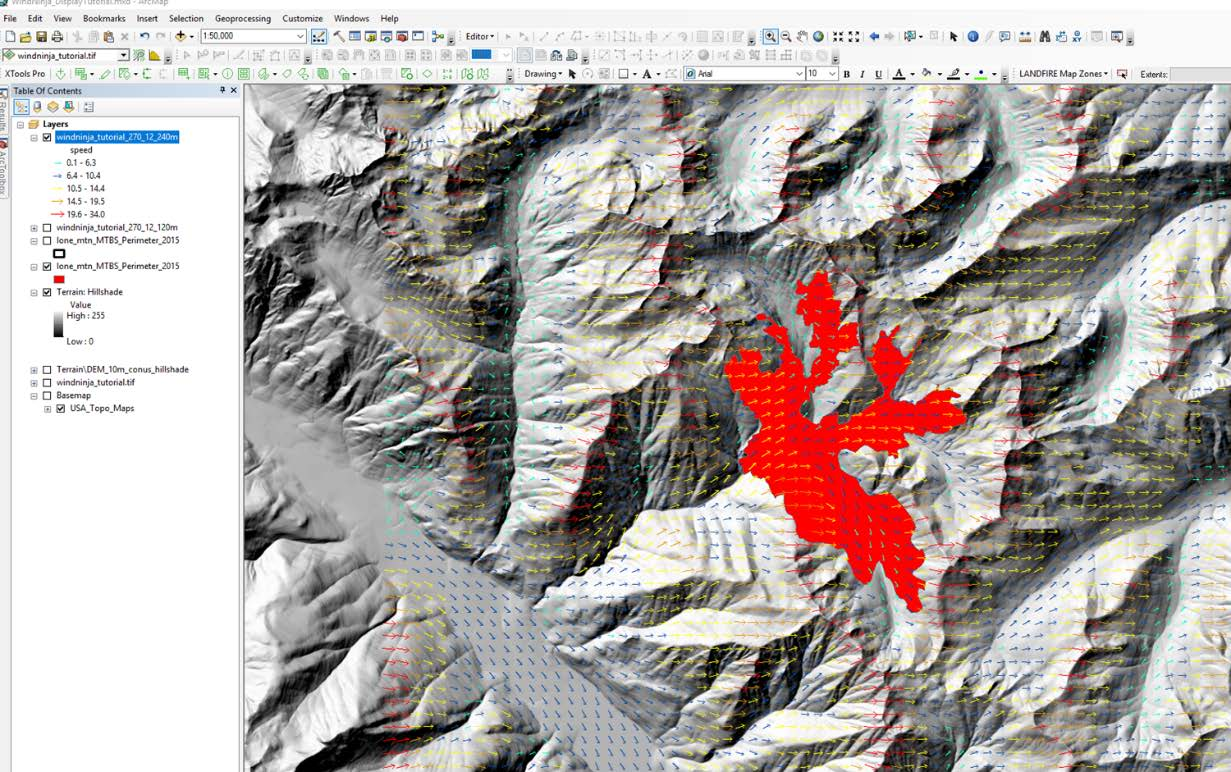
\includegraphics[scale=0.35]{arc_10.png}
	\caption{Rotated WindNinja vectors displayed in ArcMap.}
\label{fig:Figure10}
\end{figure}
\end{enumerate}

\section*{Query the Gridded Wind Output in ArcMap}
To correctly rotate the arrows in ArcMap as described above requires manipulation of the data
generated by the WindNinja software for display purposes. In Figure 11 the query information for the
circled arrow shows the wind speed as 24.3 mph with an AM\_dir of 359. The AM\_dir value for wind
direction in the shapefile \textbf{IS NOT} the same value as generated by the WindNinja software; it is for
rotation and display purposes only. For this point the wind speed is 24.3 mph (speed) and wind is
coming from 269 degrees (Dir). The values for speed and dir are the WindNinja-derived values that
should be used in any analysis using this shapefile.

\textbf{Note}: The appropriate angle file ASCII output from WindNinja will need to be converted to ESRI
GRID format in order to use the information as illustrated here.

\begin{figure}[H]
	\centering
	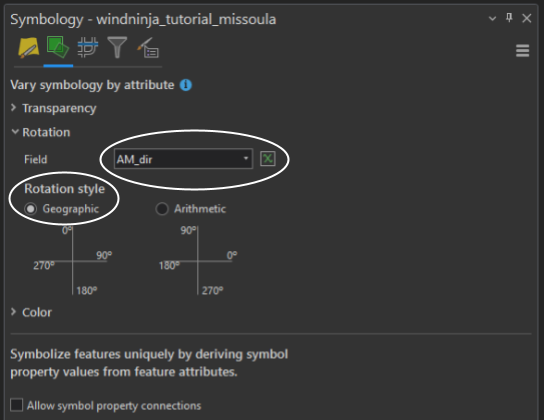
\includegraphics[scale=0.35]{arc_11.png}
	\caption{Query results of gridded wind shapefile in ArcMap showing the difference in the wind direction in the shapefile and
the rotation angle of the arrow. Query done after the shapefile has been rotated following previous steps.}
\label{fig:Figure11}
\end{figure}
\newpage
Figure~\ref{fig:Figure12} focuses on the same point on the landscape. However, in this case the ArcMap shapefile is
overlayed on the GRID of wind direction generated by the WindNinja software. A query of the individual
raster cell shows a pixel value of 269 which corresponds to the direction the wind is coming from.

\begin{figure}[H]
	\centering
	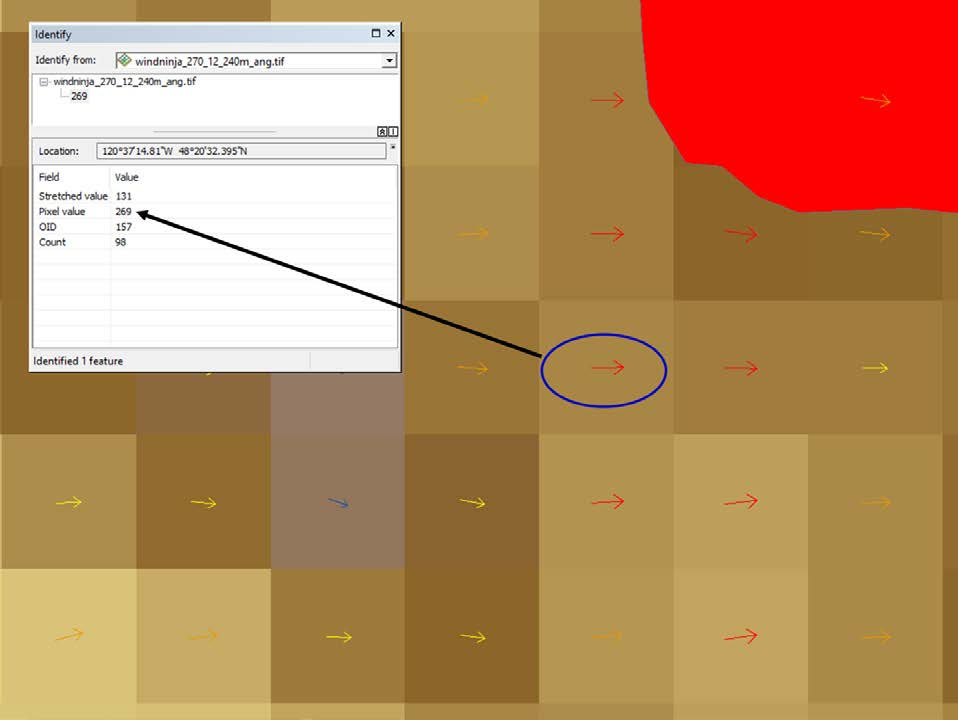
\includegraphics[scale=0.5]{arc_12.png}
	\caption{Query of the gridded wind generated ArcMap shapefile overlayed on the GRID ASCII Raster output from the WindNinja software.}
\label{fig:Figure12}
\end{figure}


\renewcommand{\thefigure}{\arabic{figure}}
\setcounter{figure}{0}

\pagebreak
\begin{centering}
\section*{Appendix}
\label{section:appendix}

\subsection*{How to Change the Number of Records Used In ArcMap when Displaying WindNinja Shapefile Output}
Chuck McHugh, RMRS, Fire Sciences Lab, Missoula, MT, 406-829-6953, \href{mailto:cmchugh@fs.fed.us}{cmchugh@fs.fed.us}.
\end{centering}
\newline
When displaying the WindNinja-derived wind direction-speed shapefile information in ArcMap, the warning
displayed in Figure~\ref{fig:Figure13} will often occur. This is because the default number of records to be displayed in ArcMap is
the \textbf{First 10,000 Records} regardless of the distribution and spatial location of the data. Depending on the output
file resolution size selected in the WindNinja software and the landscape extent, this number can easily be
exceeded. As a consequence, not all records in the shapefile will be used during display of the wind speed values.
Additionally, within ArcMap your choice of \textbf{Classification Method} and the number of \textbf{Classes} will also affect
the displayed ranges of information.
\begin{figure}[H]
	\centering
	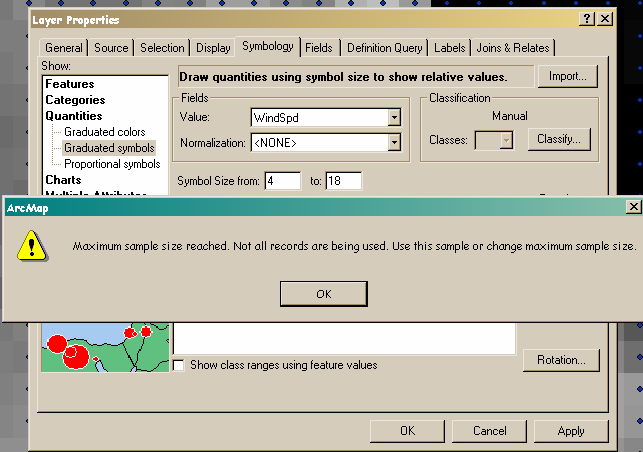
\includegraphics[scale=0.7]{arc_13.png}
	\caption{Error message when the number of records in the WindNinja ArcMap shapefile exceeds the default
settings.}
\label{fig:Figure13}
\end{figure}

Because only the first 10,000 records are used, not all of the information will be used in defining the ranges of wind
speed during the rotation process. This can lead to a misunderstanding of what the maximum and minimum wind
speed values really are. For example, in Figure~\ref{subfig:s14} the maximum wind speed value displayed is 13 mph while in
Figure~\ref{subfig:s15} the maximum wind speed value displayed is 20 mph. These statistics are based on the total number of
records used as limited by the \textbf{Number of Records} used.

\begin{figure}[H]
\centering
\subfloat[Using default setting
of 10,000 records]{
		  \label{subfig:s14}
		  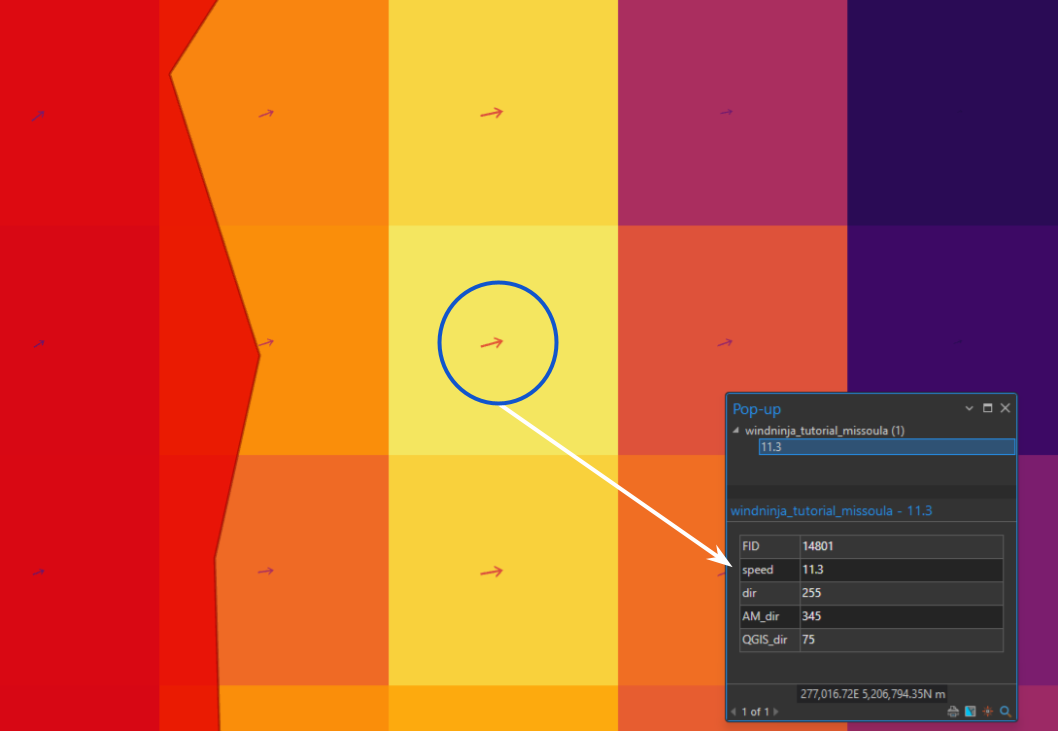
\includegraphics[scale=0.5]{arc_14.png}}\\
\subfloat[Setting Maximum Sample size so all records are used]{
		  \label{subfig:s15}
		  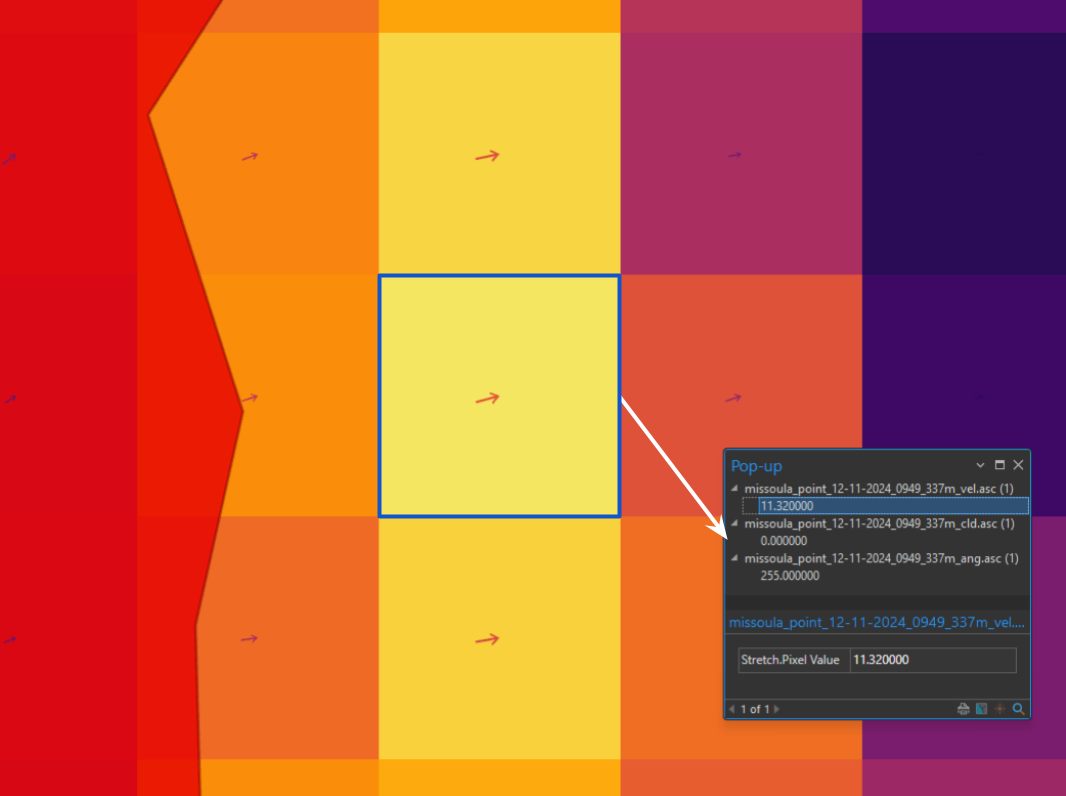
\includegraphics[scale=0.5]{arc_15.png}}
\caption{Displayed ranges of wind speed values based on Maximum Sample Size.(\ref{subfig:s14}) Using default setting
of 10,000 records and (\ref{subfig:s15}) Setting Maximum Sample size so all records are used}
\label{fig:Figure14_1}
\end{figure}

\pagebreak

To change the number of records used for the shapefile is an easy change. This is not a universal change to the
ArcMap settings but only applies to the shapefile while active in the view. Thus, every time you add this file
to another ArcMap project you will have to repeat this step. To change the settings first click on the \textbf{OK}
button in the warning message; this will remove the warning message box. Next, select \textbf{Classify} (Figure~\ref{fig:Figure16}).
Selecting the \textbf{Classify} button will open the window displayed in Figure~\ref{fig:Figure17}.

\begin{figure}[H]
	\centering
	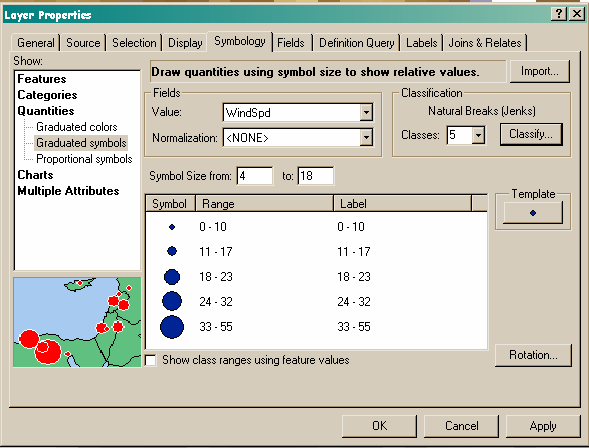
\includegraphics[scale=0.7]{arc_16.png}
	\caption{Classify button to start the process of changing the default settings for number of records displayed in
ArcMap.}
\label{fig:Figure16}
\end{figure}

\begin{figure}[H]
	\centering
	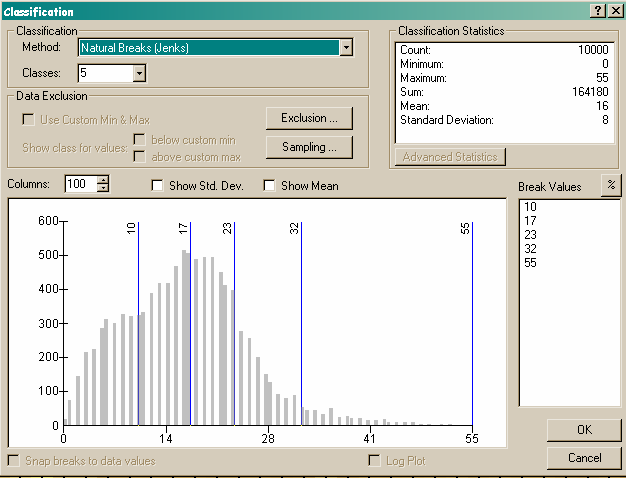
\includegraphics[scale=0.7]{arc_17.png}
	\caption{Classification window showing the number of records used in the Classification Statistics displayed in
ArcMap.}
\label{fig:Figure17}
\end{figure}

In the \textbf{Classification} Statistics pane in the upper right you can see the number of records used (Count), minimum
and maximum, mean, and standard deviation. All of these values will change based on the \textbf{Data Sampling} method
selected; in this case the number of values is the default value of \textbf{First 10,000 Records}.

\textbf{Note}: The number of records or sampling method chosen here does not affect summary or statistical operations performed on the data fields within the shapefile attribute table. Operations performed on the shapefile attribute table will use all of the records available for the selected data field unless a subset of the records has been selected.

To change the \textbf{Maximum Sampling Size}, select the \textbf{Sampling} button (Figure~\ref{fig:Figure17}). This will open the Data Sampling dialog box displayed in Figure ~\ref{fig:Figure18}.

\begin{figure}[H]
	\centering
	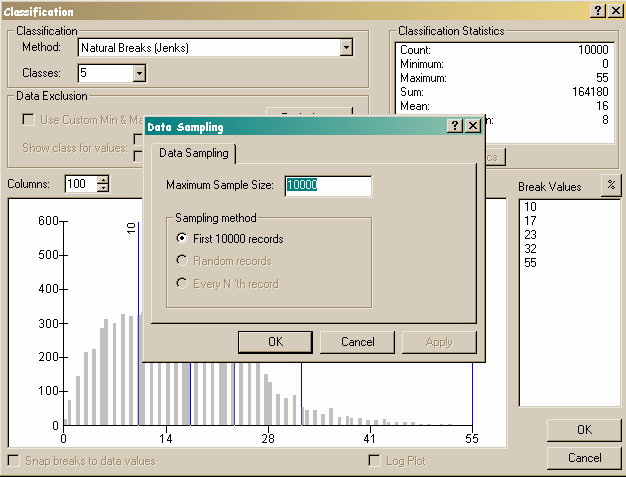
\includegraphics[scale=0.7]{arc_18.png}
	\caption{Dialog box to change the data sampling and sampling methods for the shapefile in ArcMap.}
\label{fig:Figure18}
\end{figure}

In the \textbf{Data Sampling} dialog box you will need to change the Maximum Sample Size used from 10,000 to a larger value (Figure~\ref{fig:Figure18}). After changing the \textbf{Maximum Sample Size} value click on \textbf{OK} until all dialog boxes have closed. For most shapefiles changing this value to 100,000 should ensure that all records are being used. However, the number of records included in any one shapefile is determined by the size of the landscape as well as the output resolution selected in the WindNinja software. Because of this you may need to set this value higher in some cases.

To see how many records are in the shapefile, you can do the following.
\begin{enumerate}

\item In the Table of Contents pane right-click on the shapefile of interest.
\item  Select Open Attribute Table.
\item On the bottom right-hand side will be the statement “Records (0 out of \#\# Selected). The \#\# will be the
total number of records in the shapefile (Figure~\ref{fig:Figure19}). If a subset of the total number of records has been
selected this too can be determined. The number of selected records would show up where the 0 is for this
example.

\end{enumerate}

\begin{figure}[H]
	\centering
	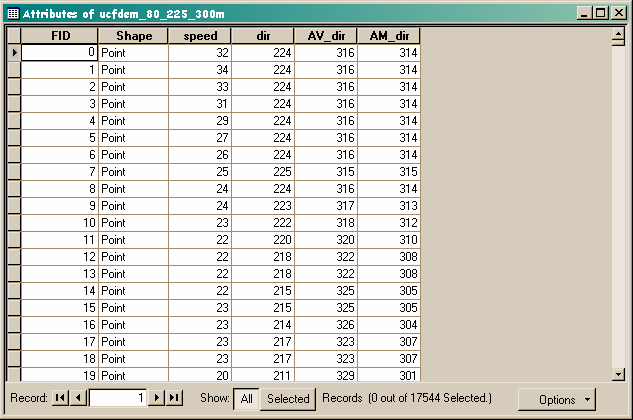
\includegraphics[scale=0.7]{arc_19.png}
	\caption{Attribute table for WindNinja-generated shapefile in ArcMap.}
\label{fig:Figure19}
\end{figure}

\end{document}